%!TEX root = ../presentation.tex
\section{Einleitung}

\begin{frame}{}{}
    EINLEITUNG HIER
\end{frame}

\subsection[nötige Funktionen]{Wasfür Funktionen sollen gewährleistet sein?}

\begin{frame}{Funktionen}
    \begin{itemize}
        \item intuitiv wie Kalender bedienbar, aber \textrightarrow  \textbf{Konfliktlösung}
        \item klar erkennbar, ob Raum frei für spontane Nutzung
        \item Möglichkeit zum Raum Teilen
        \item einfache Nutzung (mobile Endgeräte, schnell buchen, etc.)
        \item einfache Lesbarkeit für alle (alles erklärt, Darkmode)
    \end{itemize}
\end{frame}

\subsection[Werdegang und Schwierigkeiten]{Wie sind wir dahin gekommen und was waren Schwierigkeiten?}

\begin{frame}{Wie sind wir dahin gekommen?}
    \begin{itemize}
        \item Interviews zur Bedarfsanalyse
        \item Umsetzung in Treffen diskutiert
    \end{itemize}
\end{frame}

\begin{frame}
    \begin{figure}
        \centering
        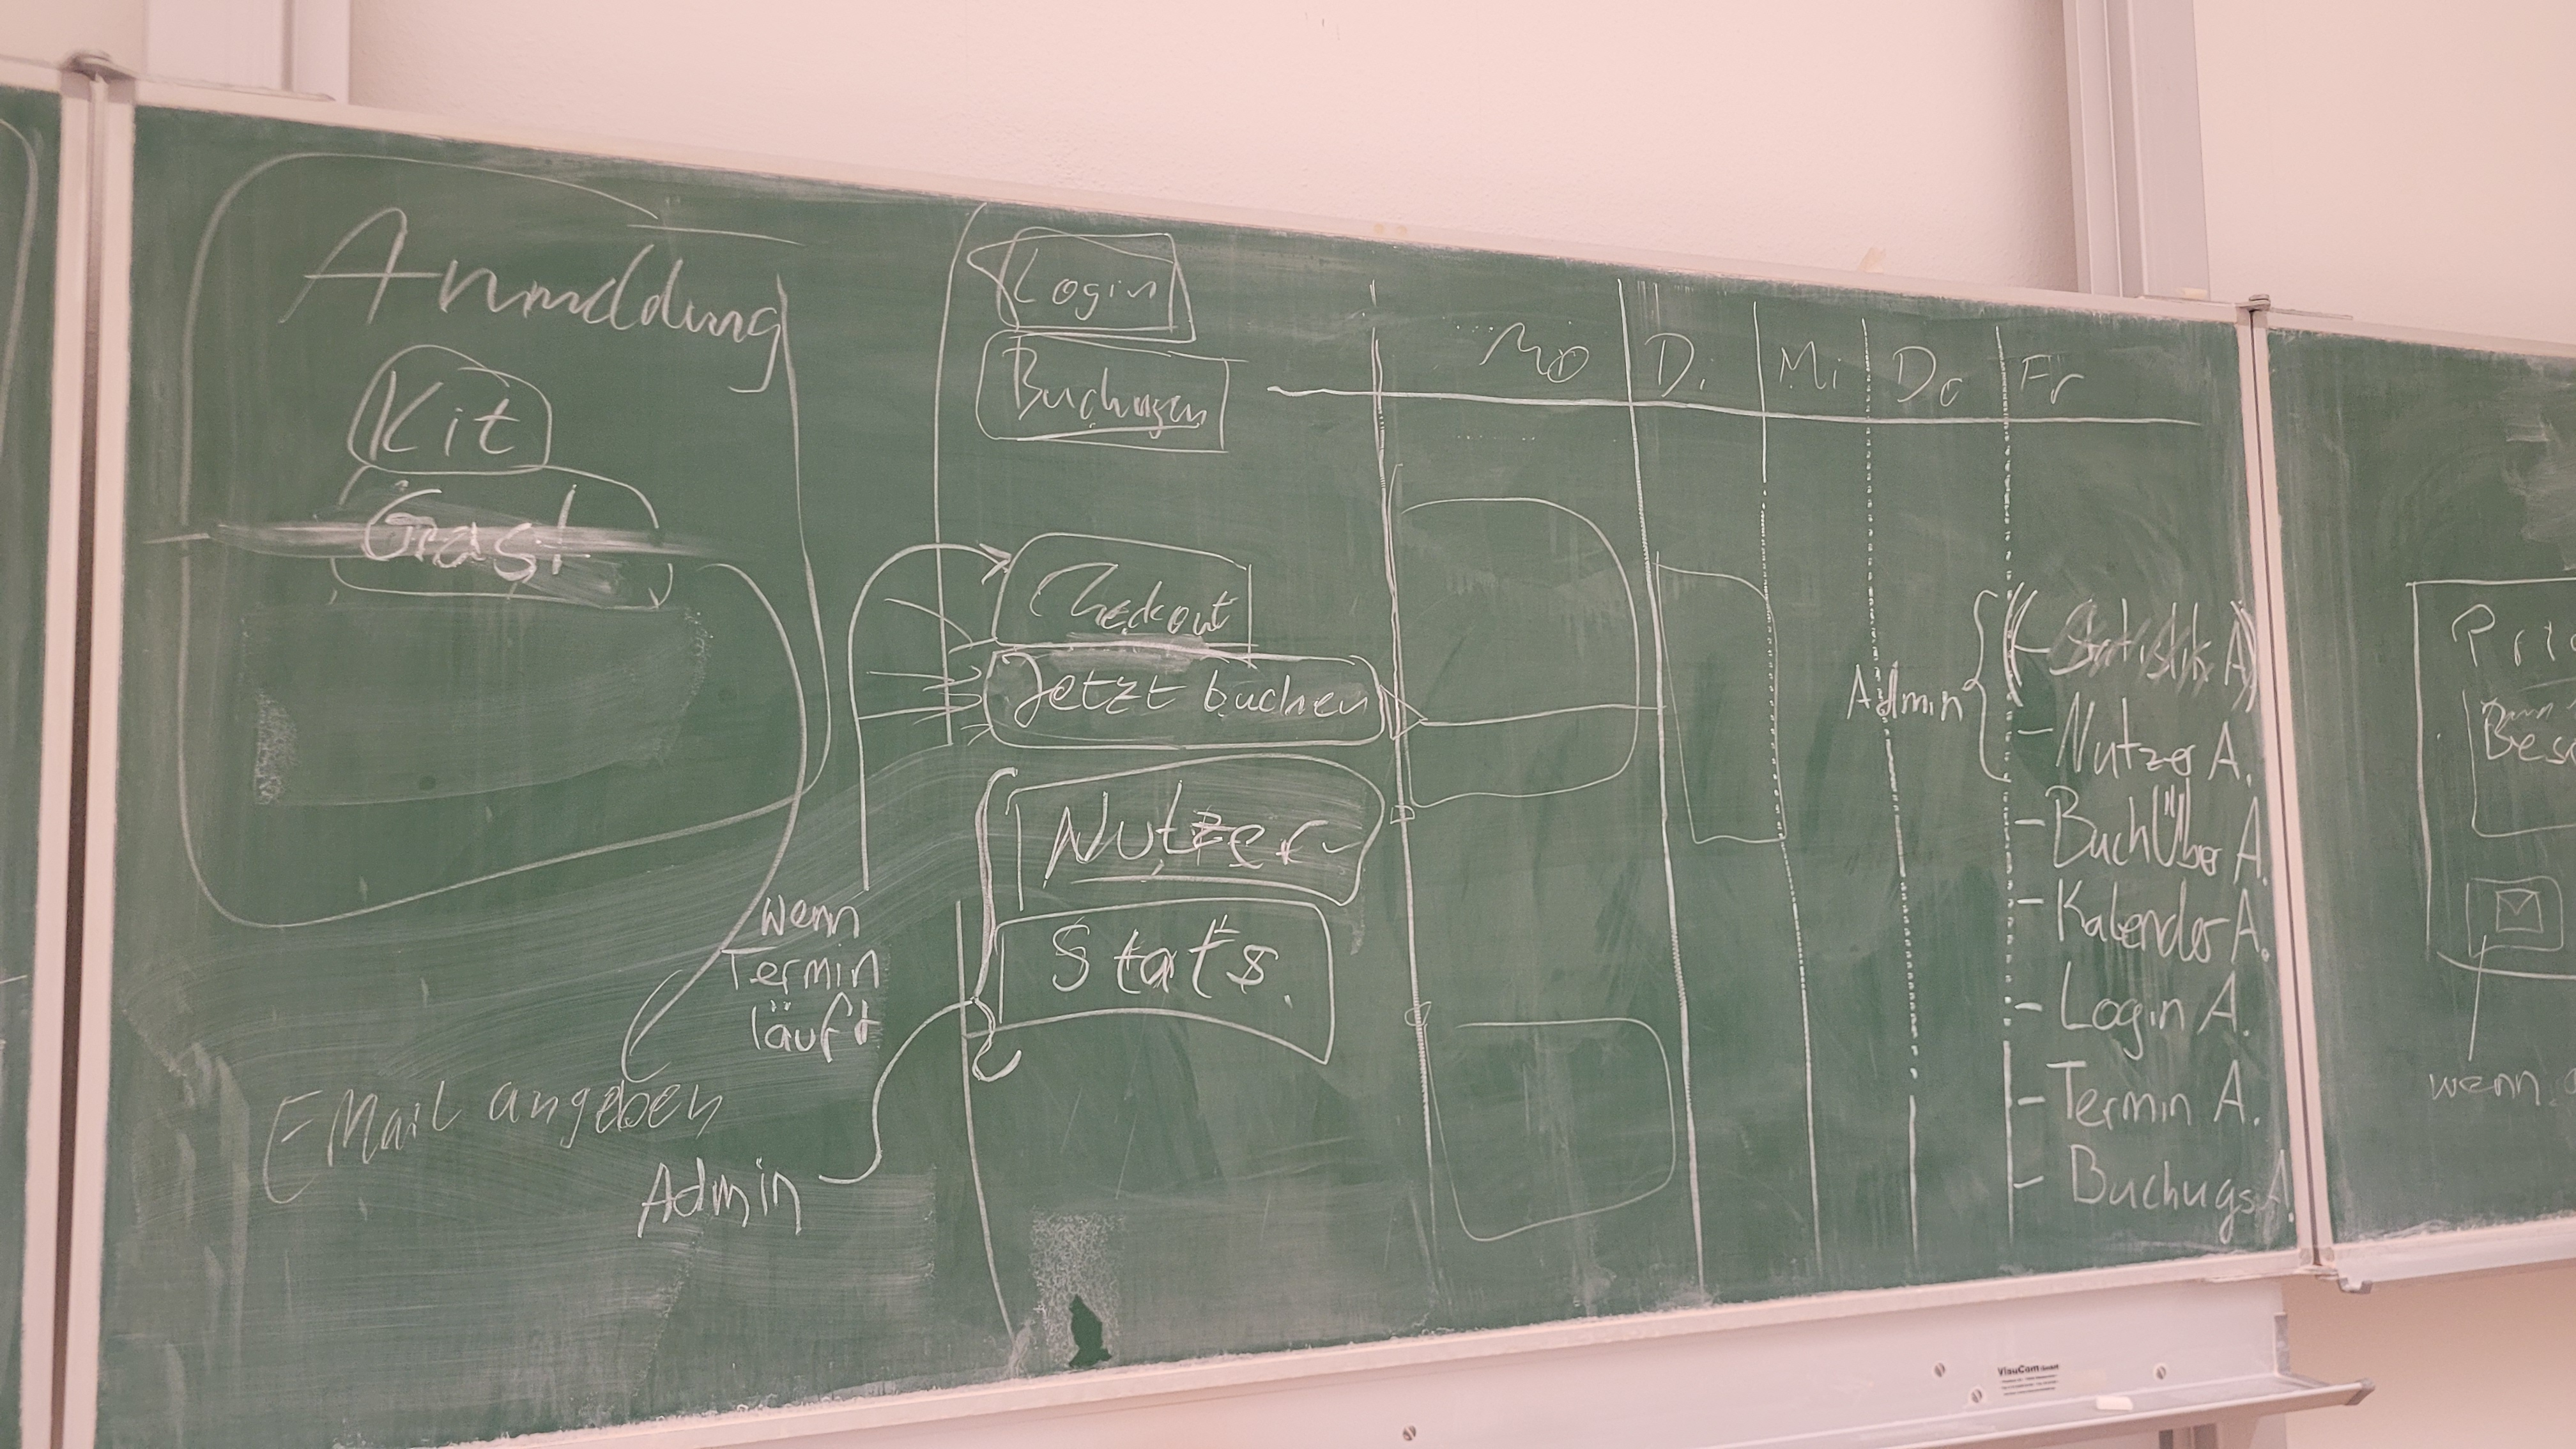
\includegraphics[width=0.6\linewidth]{pictures/BrainstormTafelbild}
        \label{fig: Tafelbild Brainstorm}
    \end{figure}
\end{frame}

\begin{frame}
    \begin{figure}
        \centering
        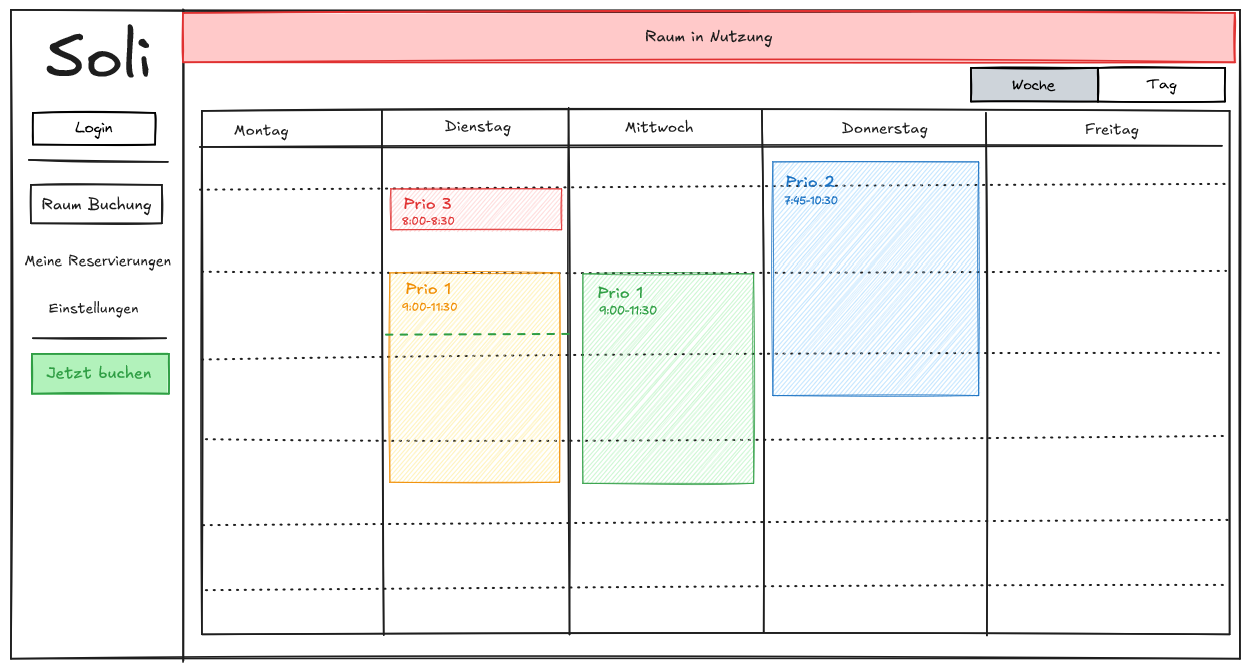
\includegraphics[width=0.6\linewidth]{pictures/BenutzeroberflächeKalender}
        \label{fig: Mockup Übersicht}
    \end{figure}
\end{frame}

\begin{frame}{Schwierigkeiten}
    \begin{itemize}
        \item Wie Konfliktlösung?
        \item Wie wird informiert oder verhandelt?
        \item Ist Hardware möglich?
    \end{itemize}
\end{frame}
